\section{Section 3 - Smoothing}

\begin{minipage}{\linewidth}
  \begin{minipage}{0.4\linewidth}
    \begin{figure}[H]
      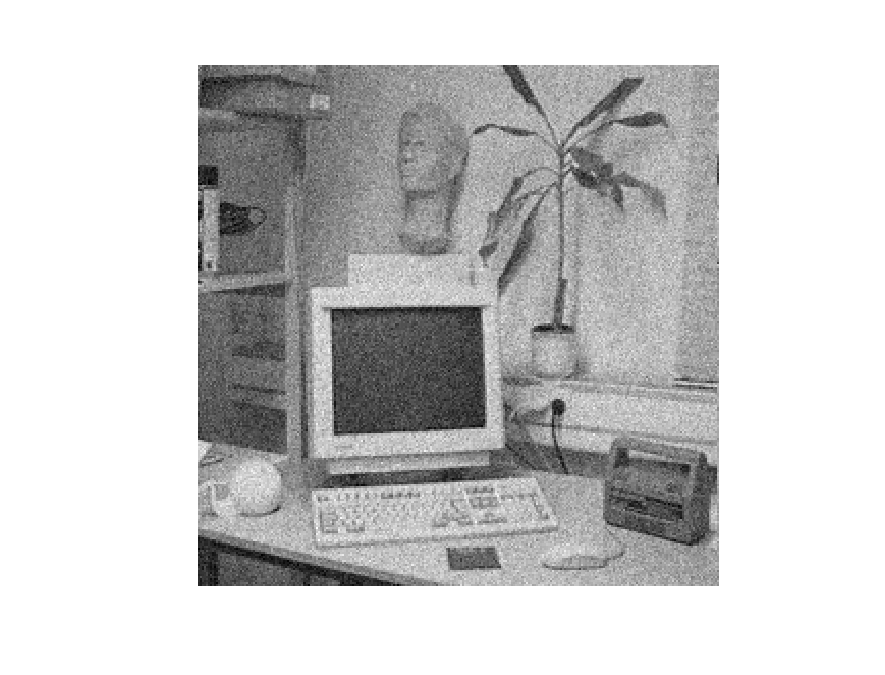
\includegraphics[scale=0.6]{./images/Q17/add_original.eps}
      \caption{Image \texttt{add}, i.e. image \texttt{office256} corrupted by white noise of $\sigma = 16$.}
      \label{fig:Q17_add_original}
    \end{figure}
  \end{minipage}
  \hspace{0.05\linewidth}
  \begin{minipage}{0.4\linewidth}
    \begin{figure}[H]
      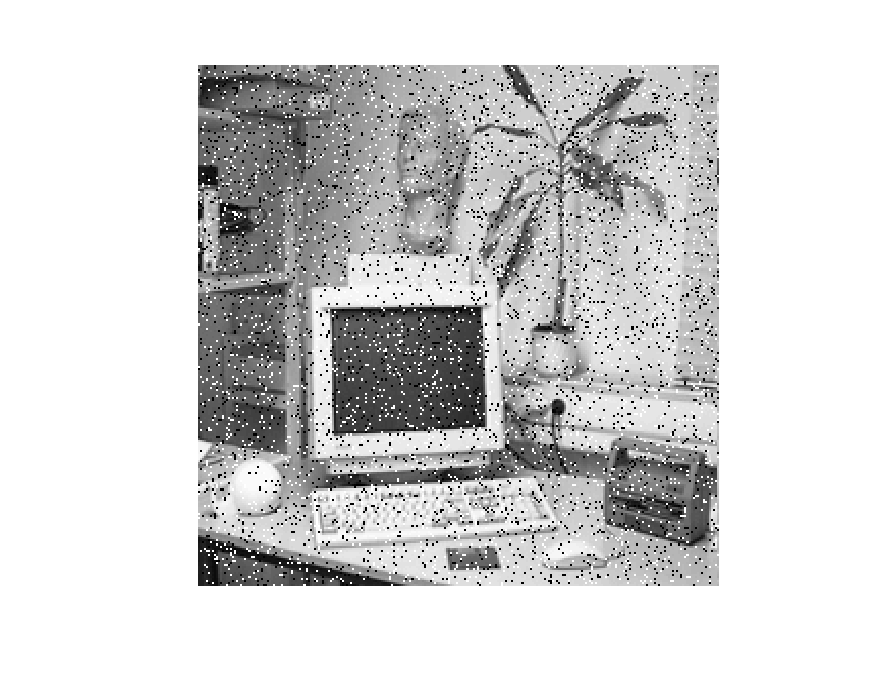
\includegraphics[scale=0.6]{./images/Q17/sap_original.eps}
      \caption{Image \texttt{sap}, i.e. \texttt{office256} corrupted by salt-and-pepper noise.}
      \label{fig:Q17_add_original}
    \end{figure}
  \end{minipage}
\end{minipage}
\\

\subsection{Question 17}

TODO

\subsubsection{Gaussian smoothing}

\begin{minipage}{\linewidth}
  \begin{minipage}{0.4\linewidth}
    \begin{figure}[H]
      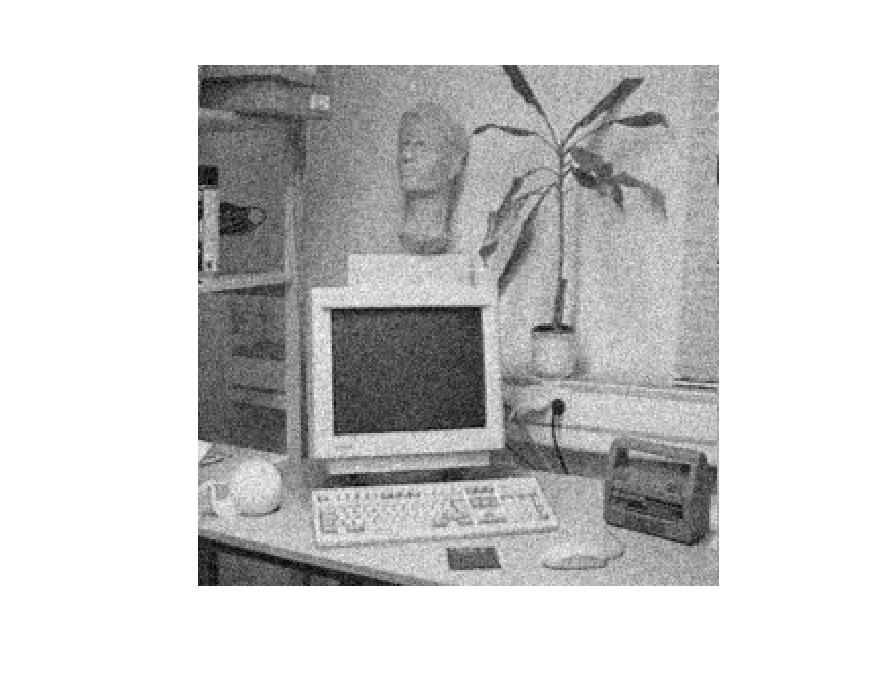
\includegraphics[scale=0.6]{./images/Q17/discgaussfft/add_01.eps}
      \caption{Smoothing of image \texttt{add} using a gaussian low pass filter of $\sigma^2 = 0.1$.}
      \label{fig:Q17_discgaussfft_add_01}
    \end{figure}
  \end{minipage}
  \hspace{0.05\linewidth}
  \begin{minipage}{0.4\linewidth}
    \begin{figure}[H]
      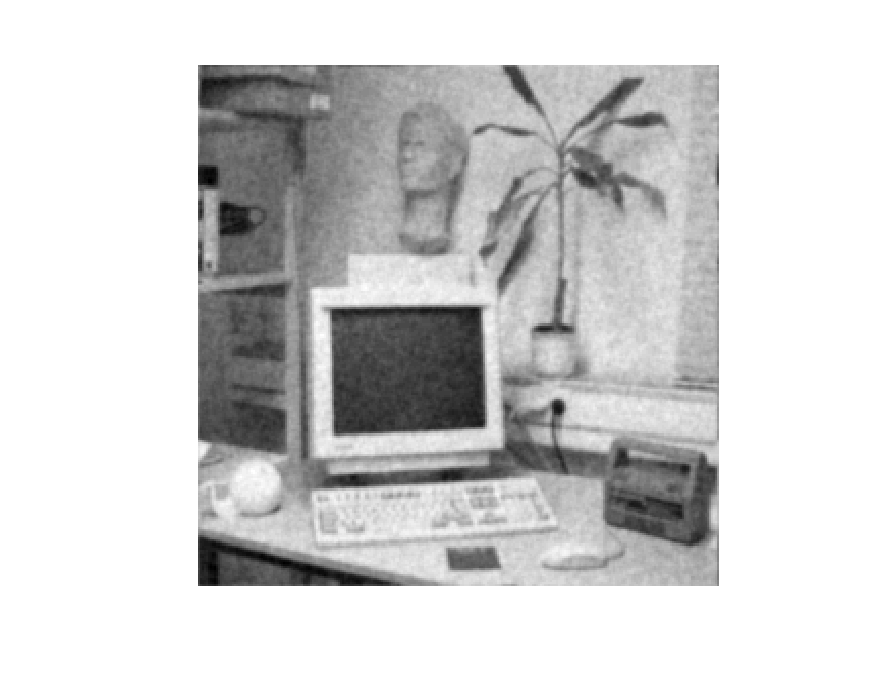
\includegraphics[scale=0.6]{./images/Q17/discgaussfft/add_1.eps}
      \caption{Smoothing of image \texttt{add} using a gaussian low pass filter of $\sigma^2 = 1$.}
      \label{fig:Q17_discgaussfft_add_1}
    \end{figure}
  \end{minipage}
\end{minipage}
\\

\begin{minipage}{\linewidth}
  \begin{minipage}{0.4\linewidth}
    \begin{figure}[H]
      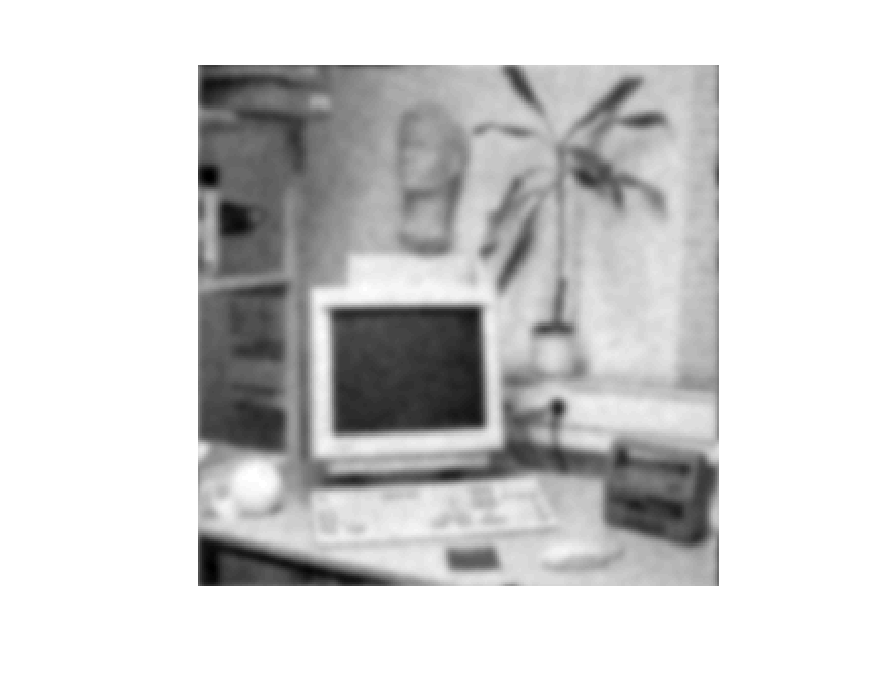
\includegraphics[scale=0.6]{./images/Q17/discgaussfft/add_4.eps}
      \caption{Smoothing of image \texttt{add} using a gaussian low pass filter of $\sigma^2 = 4$.}
      \label{fig:Q17_discgaussfft_add_4}
    \end{figure}
  \end{minipage}
  \hspace{0.05\linewidth}
  \begin{minipage}{0.4\linewidth}
    \begin{figure}[H]
      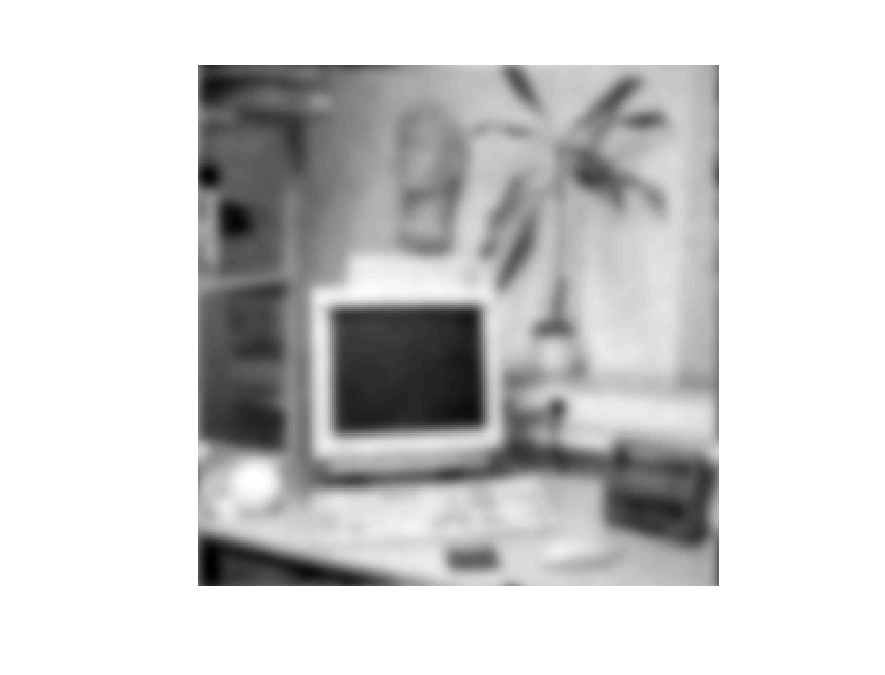
\includegraphics[scale=0.6]{./images/Q17/discgaussfft/add_10.eps}
      \caption{Smoothing of image \texttt{add} using a gaussian low pass filter of $\sigma^2 = 10$.}
      \label{fig:Q17_discgaussfft_add_10}
    \end{figure}
  \end{minipage}
\end{minipage}
\\


\begin{minipage}{\linewidth}
  \begin{minipage}{0.4\linewidth}
    \begin{figure}[H]
      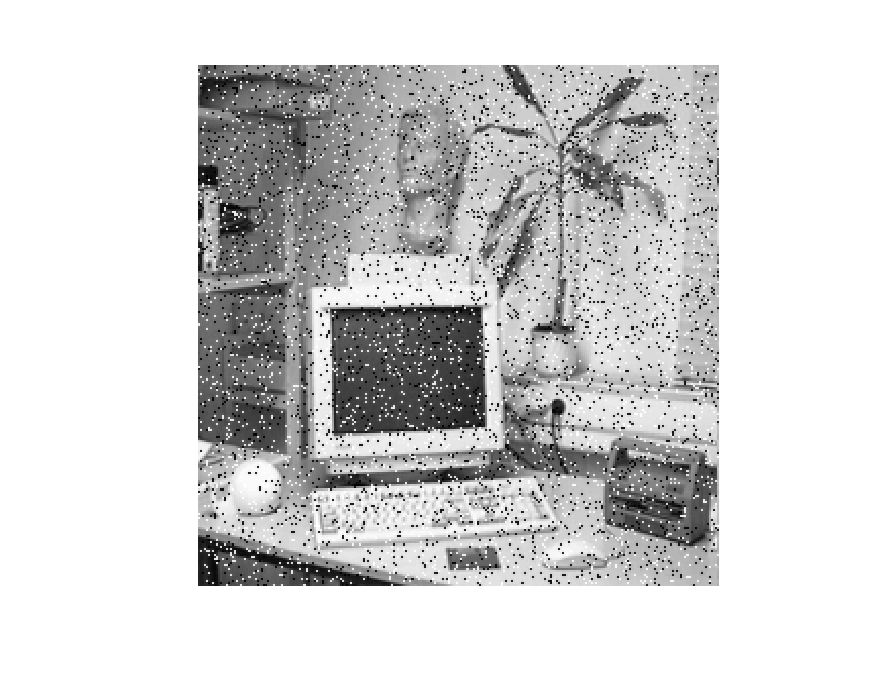
\includegraphics[scale=0.6]{./images/Q17/discgaussfft/sap_01.eps}
      \caption{Smoothing of image \texttt{sap} using a gaussian low pass filter of $\sigma^2 = 0.1$.}
      \label{fig:Q17_discgaussfft_sap_01}
    \end{figure}
  \end{minipage}
  \hspace{0.05\linewidth}
  \begin{minipage}{0.4\linewidth}
    \begin{figure}[H]
      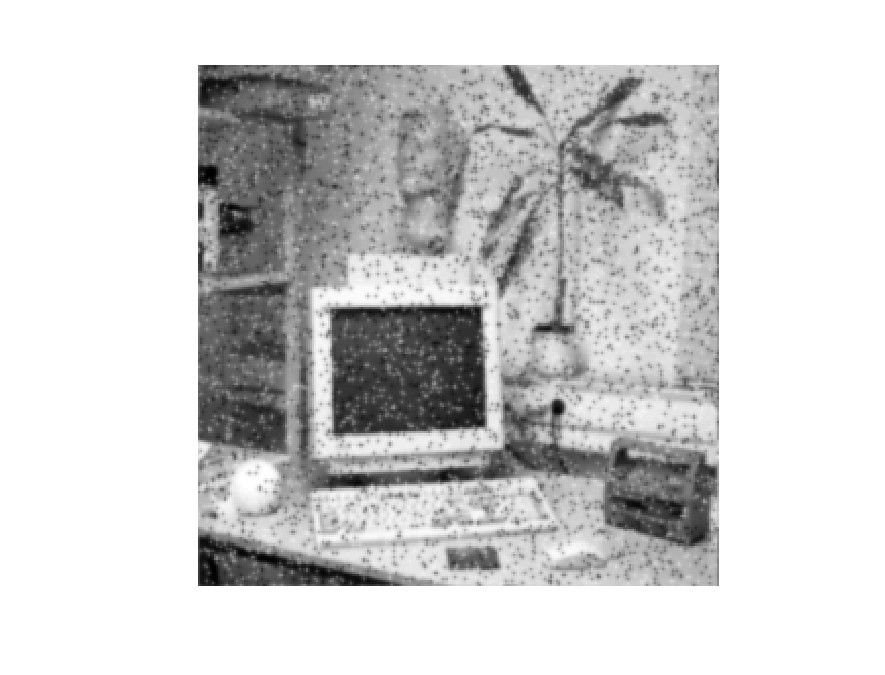
\includegraphics[scale=0.6]{./images/Q17/discgaussfft/sap_1.eps}
      \caption{Smoothing of image \texttt{sap} using a gaussian low pass filter of $\sigma^2 = 1$.}
      \label{fig:Q17_discgaussfft_sap_1}
    \end{figure}
  \end{minipage}
\end{minipage}
\\

\begin{minipage}{\linewidth}
  \begin{minipage}{0.4\linewidth}
    \begin{figure}[H]
      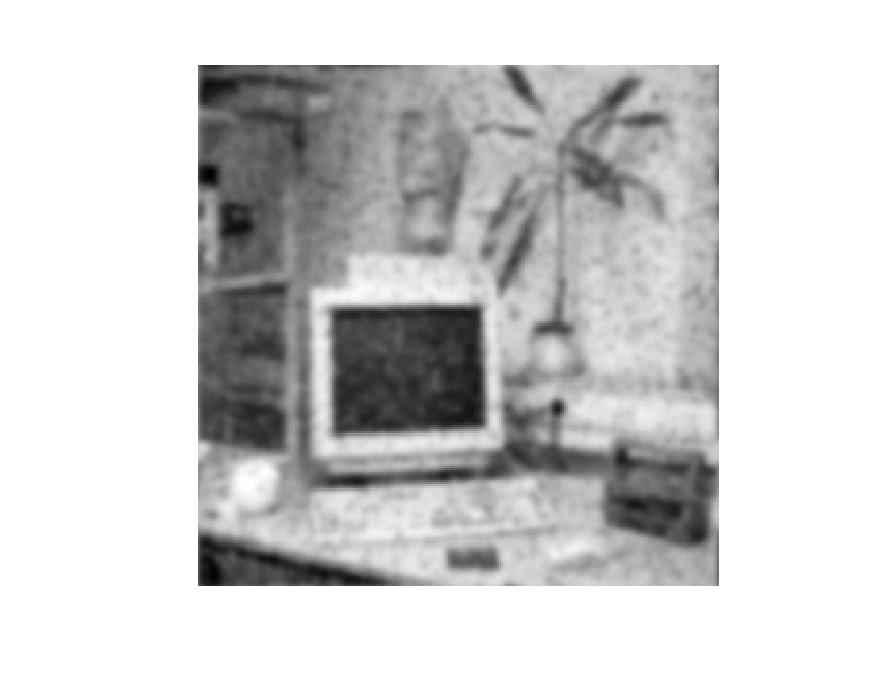
\includegraphics[scale=0.6]{./images/Q17/discgaussfft/sap_4.eps}
      \caption{Smoothing of image \texttt{sap} using a gaussian low pass filter of $\sigma^2 = 4$.}
      \label{fig:Q17_discgaussfft_sap_4}
    \end{figure}
  \end{minipage}
  \hspace{0.05\linewidth}
  \begin{minipage}{0.4\linewidth}
    \begin{figure}[H]
      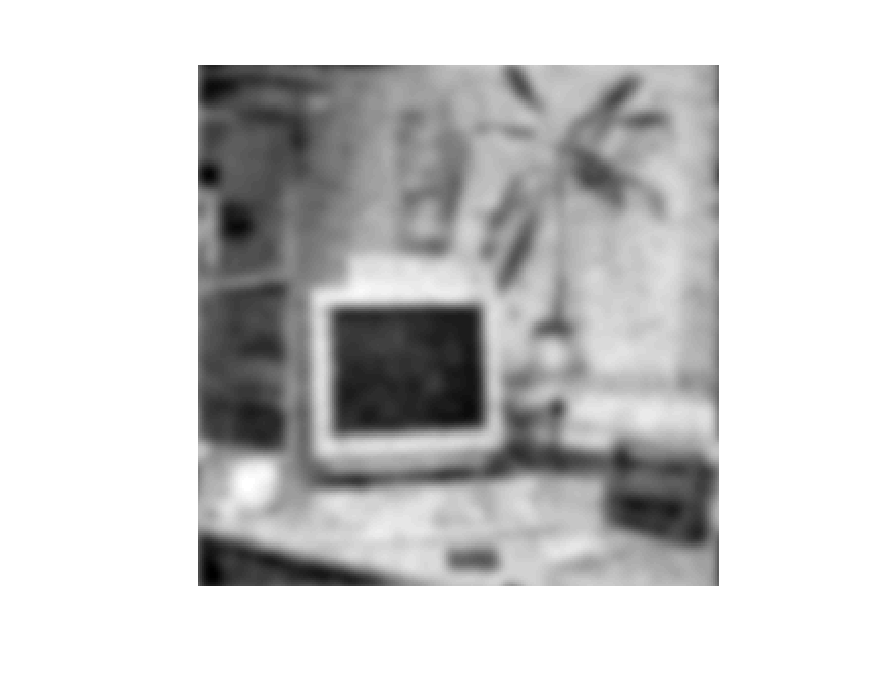
\includegraphics[scale=0.6]{./images/Q17/discgaussfft/sap_10.eps}
      \caption{Smoothing of image \texttt{sap} using a gaussian low pass filter of $\sigma^2 = 10$.}
      \label{fig:Q17_discgaussfft_sap_10}
    \end{figure}
  \end{minipage}
\end{minipage}
\\



\subsubsection{Median filtering}

\begin{minipage}{\linewidth}
  \begin{minipage}{0.4\linewidth}
    \begin{figure}[H]
      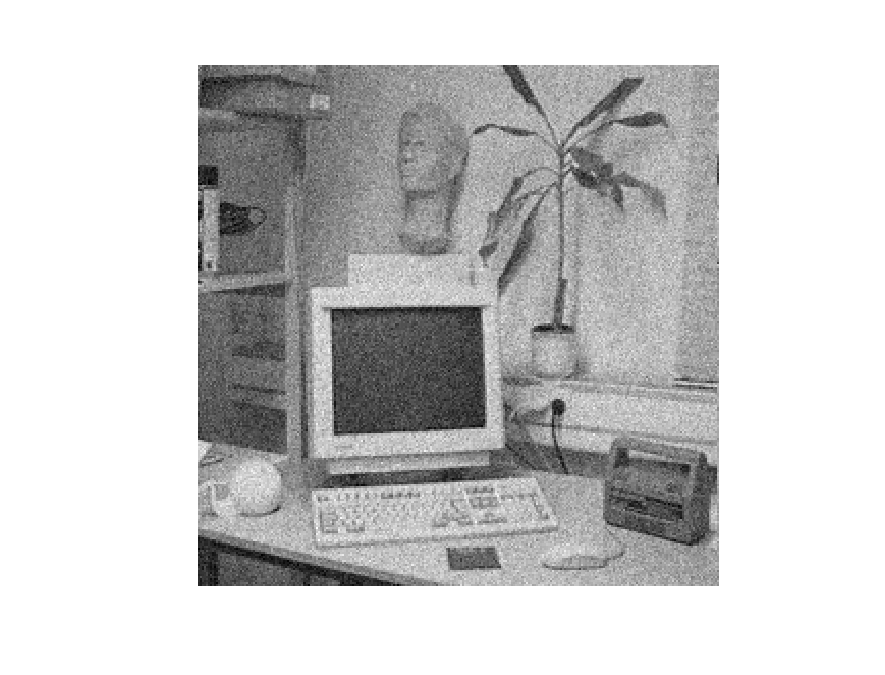
\includegraphics[scale=0.6]{./images/Q17/medfilt/add_1.eps}
      \caption{Smoothing of image \texttt{add} using a median filter of $size=1$.}
      \label{fig:Q17_medfilt_add_1}
    \end{figure}
  \end{minipage}
  \hspace{0.05\linewidth}
  \begin{minipage}{0.4\linewidth}
    \begin{figure}[H]
      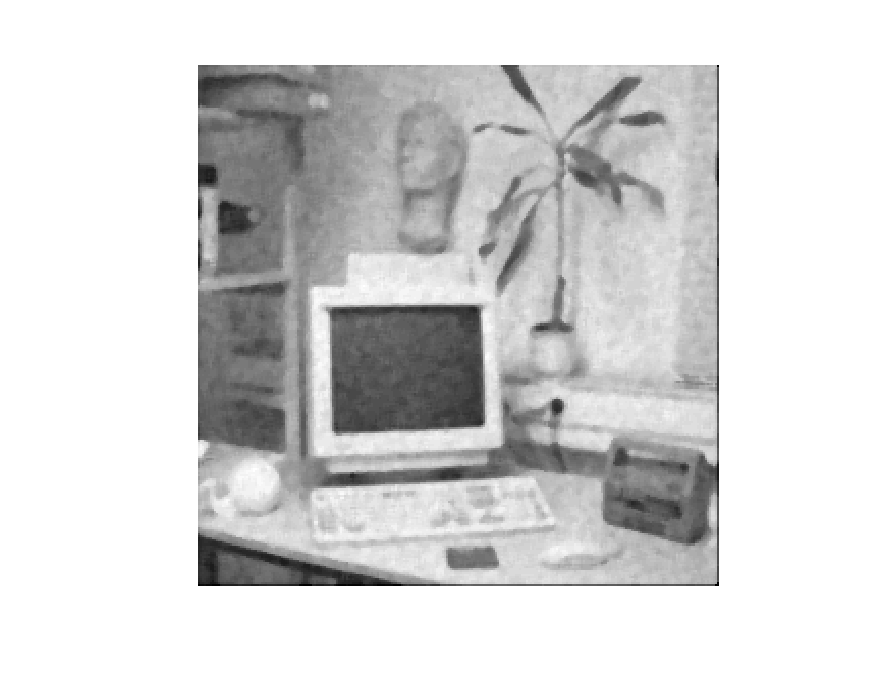
\includegraphics[scale=0.6]{./images/Q17/medfilt/add_4.eps}
      \caption{Smoothing of image \texttt{add} using a median filter of $size=4$.}
      \label{fig:Q17_medfilt_add_4}
    \end{figure}
  \end{minipage}
\end{minipage}
\\

\begin{minipage}{\linewidth}
  \begin{minipage}{0.4\linewidth}
    \begin{figure}[H]
      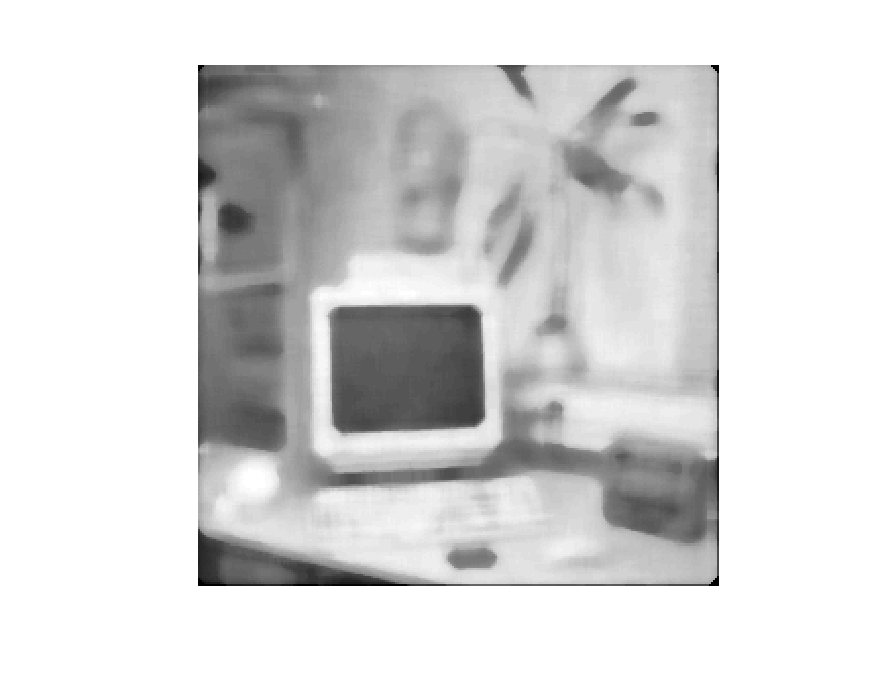
\includegraphics[scale=0.6]{./images/Q17/medfilt/add_10.eps}
      \caption{Smoothing of image \texttt{add} using a median filter of $size=10$.}
      \label{fig:Q17_medfilt_add_10}
    \end{figure}
  \end{minipage}
  \hspace{0.05\linewidth}
  \begin{minipage}{0.4\linewidth}
    \begin{figure}[H]
      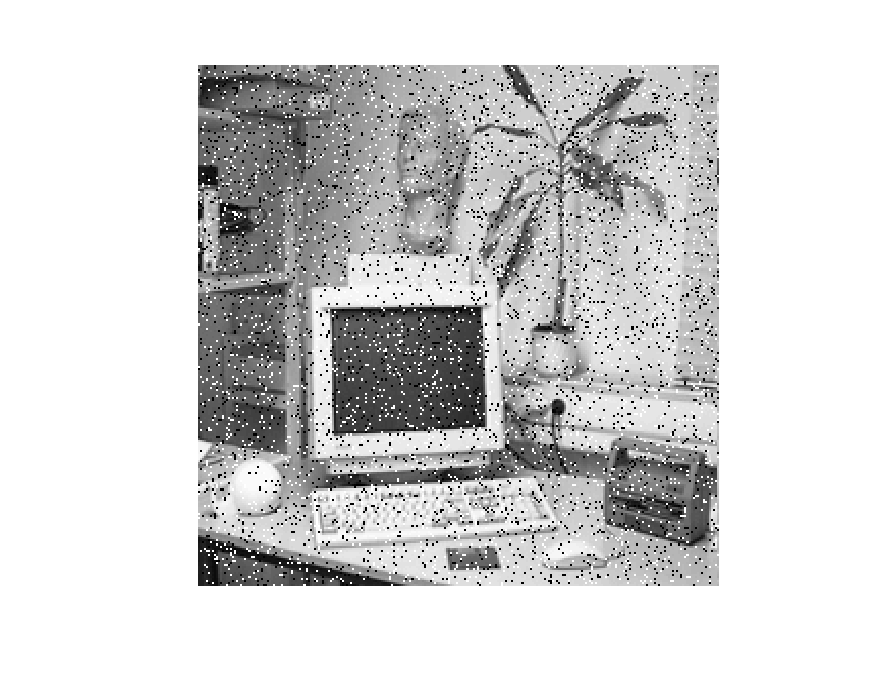
\includegraphics[scale=0.6]{./images/Q17/medfilt/sap_1.eps}
      \caption{Smoothing of image \texttt{sap} using a median filter of $size=1$.}
      \label{fig:Q17_medfilt_sap_1}
    \end{figure}
  \end{minipage}
\end{minipage}
\\


\begin{minipage}{\linewidth}
  \begin{minipage}{0.4\linewidth}
    \begin{figure}[H]
      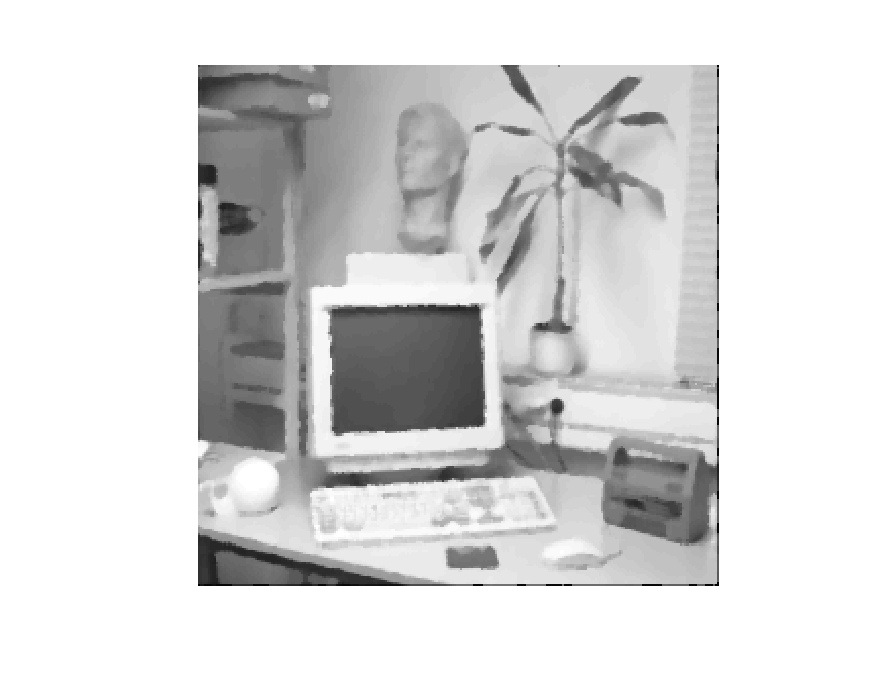
\includegraphics[scale=0.6]{./images/Q17/medfilt/sap_4.eps}
      \caption{Smoothing of image \texttt{sap} using a median filter of $size=4$.}
      \label{fig:Q17_medfilt_sap_4}
    \end{figure}
  \end{minipage}
  \hspace{0.05\linewidth}
  \begin{minipage}{0.4\linewidth}
    \begin{figure}[H]
      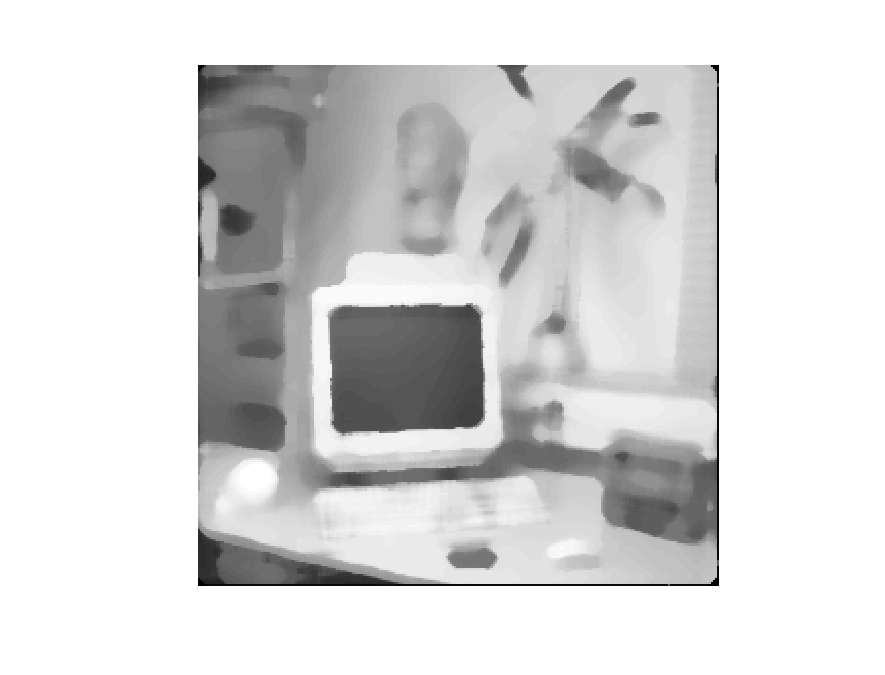
\includegraphics[scale=0.6]{./images/Q17/medfilt/sap_10.eps}
      \caption{Smoothing of image \texttt{sap} using a median filter of $size=10$.}
      \label{fig:Q17_medfilt_sap_10}
    \end{figure}
  \end{minipage}
\end{minipage}
\\



\subsubsection{Ideal low-pass filtering}

\begin{minipage}{\linewidth}
  \begin{minipage}{0.4\linewidth}
    \begin{figure}[H]
      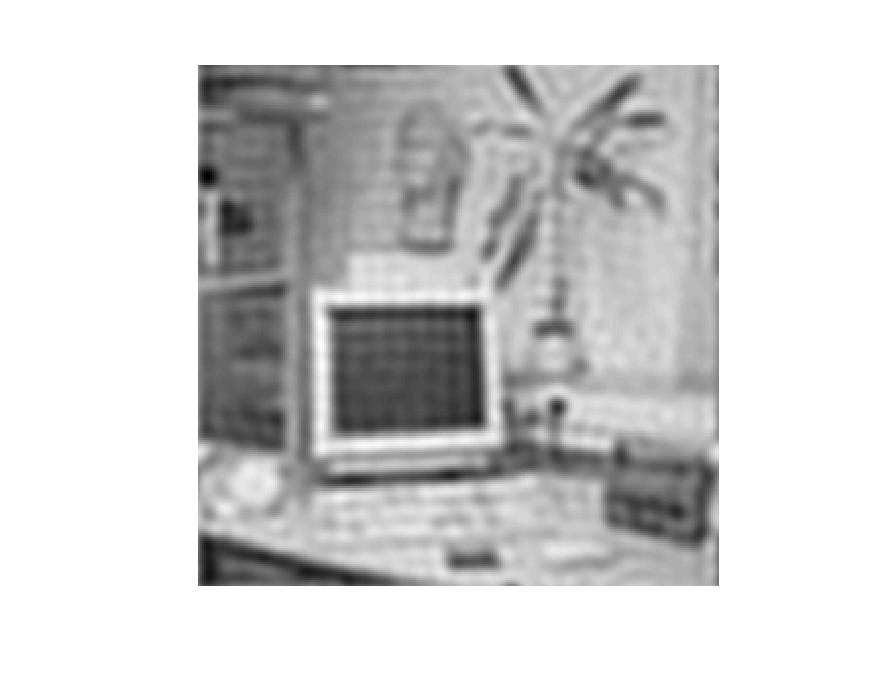
\includegraphics[scale=0.5]{./images/Q17/ideal/add_01.eps}
      \caption{Smoothing of image \texttt{add} using an ideal low-pass filter with cut-off frequency of $0.1$ cycles per pixel.}
      \label{fig:Q17_ideal_add_01}
    \end{figure}
  \end{minipage}
  \hspace{0.05\linewidth}
  \begin{minipage}{0.4\linewidth}
    \begin{figure}[H]
      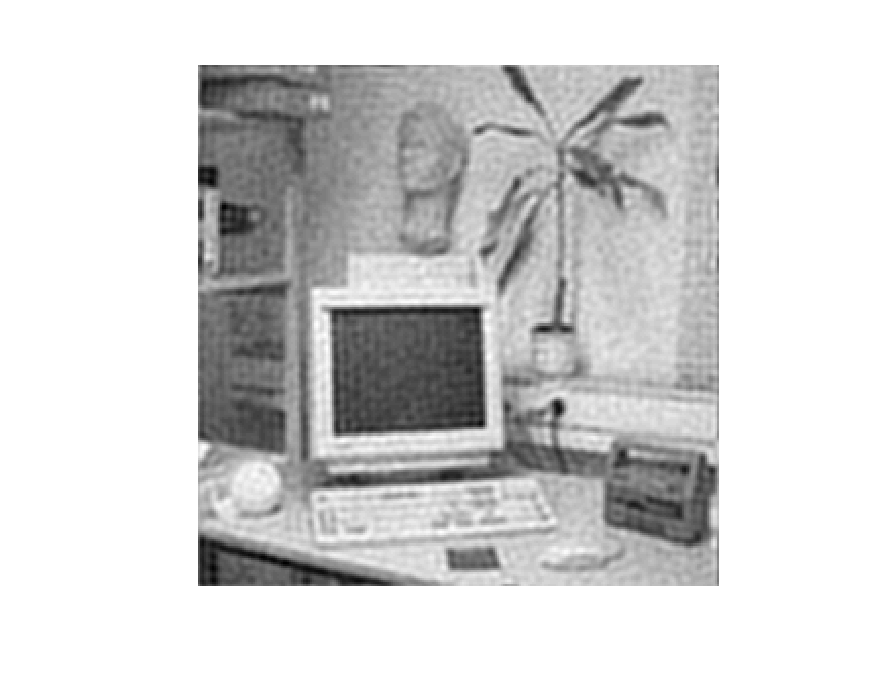
\includegraphics[scale=0.5]{./images/Q17/ideal/add_02.eps}
      \caption{Smoothing of image \texttt{add} using an ideal low-pass filter with cut-off frequency of $0.4$ cycles per pixel.}
      \label{fig:Q17_ideal_add_02}
    \end{figure}
  \end{minipage}
\end{minipage}
\\

\begin{minipage}{\linewidth}
  \begin{minipage}{0.4\linewidth}
    \begin{figure}[H]
      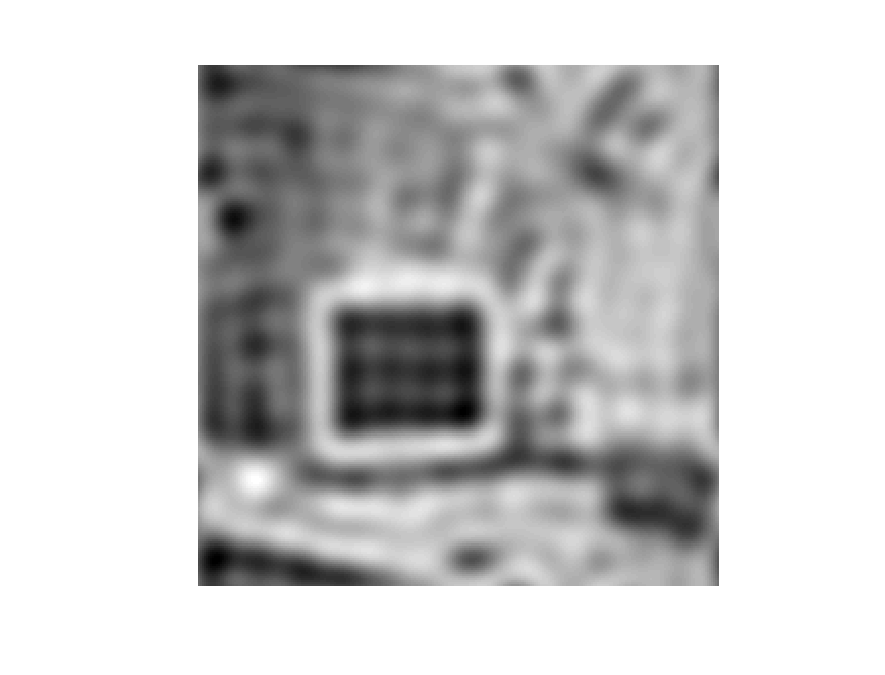
\includegraphics[scale=0.5]{./images/Q17/ideal/add_005.eps}
      \caption{Smoothing of image \texttt{add} using an ideal low-pass filter with cut-off frequency of $0.05$ cycles per pixel.}
      \label{fig:Q17_ideal_add_005}
    \end{figure}
  \end{minipage}
  \hspace{0.05\linewidth}
  \begin{minipage}{0.4\linewidth}
    \begin{figure}[H]
      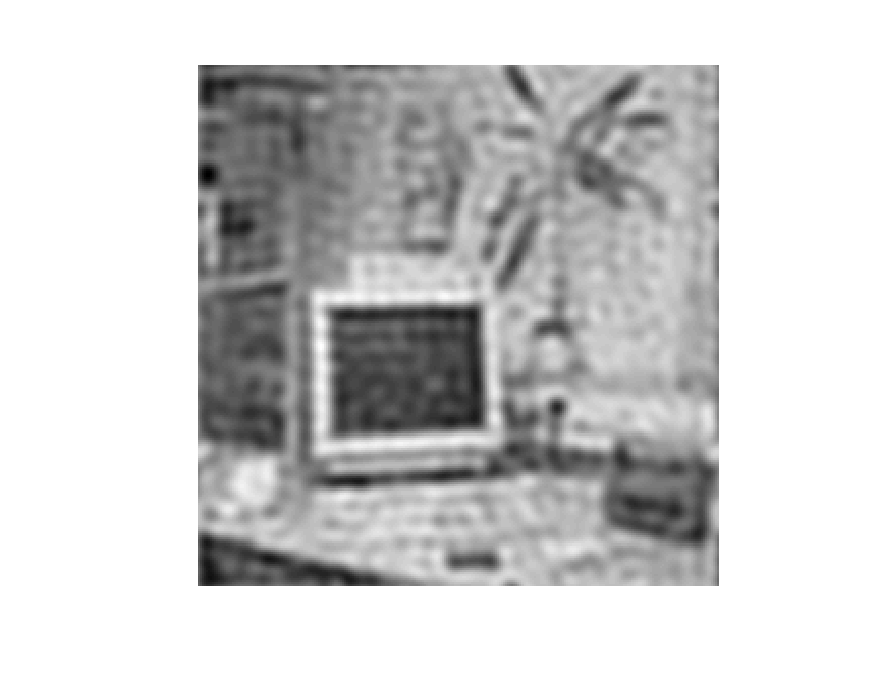
\includegraphics[scale=0.5]{./images/Q17/ideal/sap_01.eps}
      \caption{Smoothing of image \texttt{sap} using an ideal low-pass filter with cut-off frequency of $0.11$ cycles per pixel.}
      \label{fig:Q17_ideal_sap_01}
    \end{figure}
  \end{minipage}
\end{minipage}
\\


\begin{minipage}{\linewidth}
  \begin{minipage}{0.4\linewidth}
    \begin{figure}[H]
      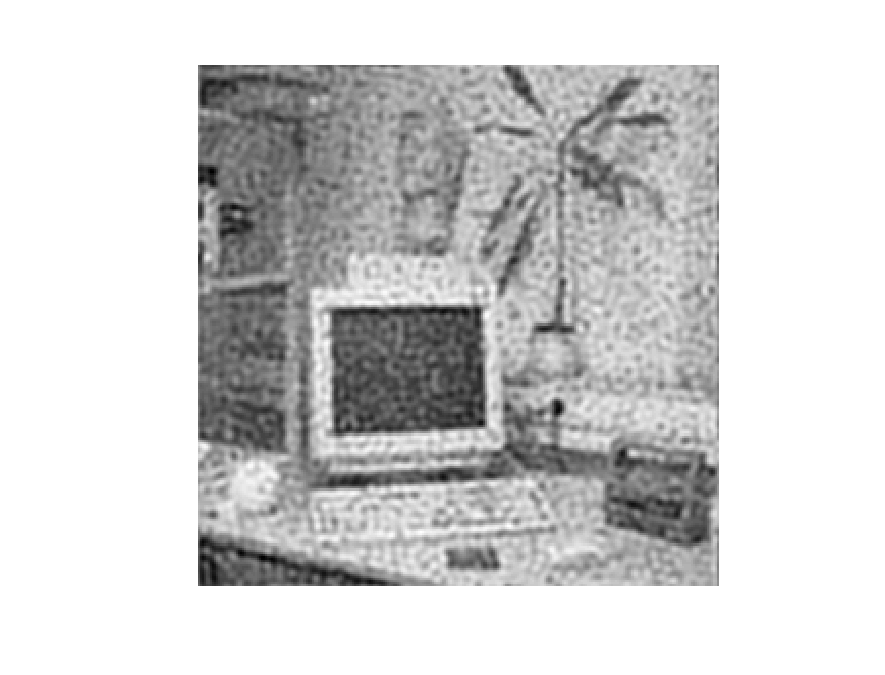
\includegraphics[scale=0.5]{./images/Q17/ideal/sap_02.eps}
      \caption{Smoothing of image \texttt{sap} using an ideal low-pass filter with cut-off frequency of $0.2$ cycles per pixel.}
      \label{fig:Q17_ideal_sap_02}
    \end{figure}
  \end{minipage}
  \hspace{0.05\linewidth}
  \begin{minipage}{0.4\linewidth}
    \begin{figure}[H]
      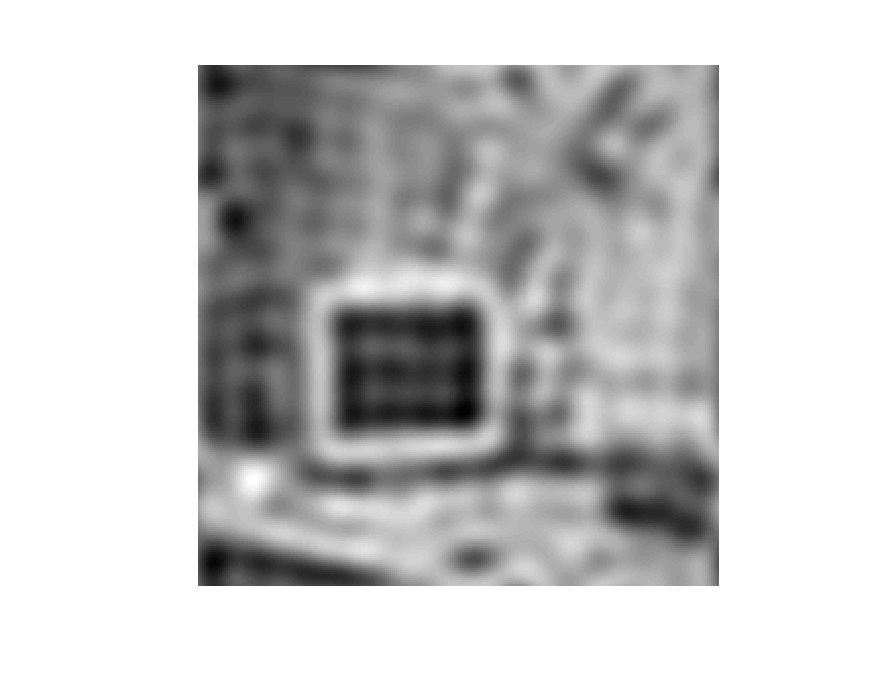
\includegraphics[scale=0.5]{./images/Q17/ideal/sap_005.eps}
      \caption{Smoothing of image \texttt{sap} using an ideal low-pass filter with cut-off frequency of $0.05$ cycles per pixel.}
      \label{fig:Q17_ideal_sap_005}
    \end{figure}
  \end{minipage}
\end{minipage}
\\


\subsection{Question 18}

TODO
